\section{Overview}

Using the detected energy per strokes of the World Wide Lightning Location Network (WWLLN) we calculate the relative detection efficiency for the network as if it had a uniform  detection efficiency.
The model uses the energy statistics of located strokes to determine which stations are sensitive to what stroke energies.
We are then able to estimate the number of strokes that may be missing from any given regions as compared to the best, most sensitive regions of the WWLLN network.
Stroke density maps can be corrected with the knowledge of how sensitive various regions of the network are operating.

This new model for the relative WWLLN detection efficiency compensates for the uneven global coverage of the network sensors as well as variations in very low frequency (VLF) propagation.
The model gives a way to represent the global distribution of strokes as if observed by a globally uniform network.
The model results are analyzed in spatial and temporal regimes, and the effects of a single VLF detector going offline are investigated in areas of sparse and dense detector coverage.
The results are also used to show spatial, temporal and energy distributions as seen by the detection efficiency corrected WWLLN.

The WWLLN network does not observe lightning with the same detection efficiency everywhere.
This is due to variable WWLLN station coverage and the strong effect on very low frequency (VLF) radio propagation from orography and ionospheric conditions along the great circle path of a wave.
This paper demonstrates a technique which uses only data collected by the WWLLN network itself, to estimate the relative detection efficiency of each $5^\circ$ x $5^\circ$ pixel over the earth compared to the best average WWLLN detection efficiency.
For instance, the lightning stroke density over central Africa, where WWLLN station density is sparse, can now be compared to the region of the Earth with the best detection efficiency, such as North America.
This chapter does not provide an absolute detection efficiency calculation.

A concern for all VLF networks is the non-uniform propagation of VLF waves due to changing ionospheric  and surface conditions; this is true for networks monitoring lightning produced VLF signals like WWLLN, or those monitoring fixed-frequency communication transmitters like AARDDVARK \citep{Clilverd2009}.
During the day there is a larger ionospheric electron density at lower D-region altitudes.
This causes the range of electron-neutral collision frequencies to overlap with the range of sferic wave frequencies, increasing the attenuation rate of the sferics.
This increase in electron number density is also seen in the change of the reference ionospheric height, $h'$ \citep{Wait1960a}, during the day ($h'=74$~km) compared to during the night ($h'=87$~km).
There is a similar change in attenuation over the path of the sferic from the differences in the conductivity of the oceans (4~S/m), continents ($10^{-2}$~-- $10^{-4}$~S/m), and Antarctic/Arctic ice ($10^{-5}$~S/m).
The many path parameters for a given sferic result in a highly variable attenuation \citep{Volland1995}.

Thus, independently determining the real-time detection efficiency has always been a challenging topic.
Several studies have been conducted comparing WWLLN to other ground based networks or satellite measurements \citep{Lay2004b, Jacobson2006c, Rodger2009, Abarca2010, Abreu2010}.
These studies tend to be limited in either scope or in time due to the availability of data from other lightning derection networks.
Past work by \citet{Rodger2006} attempted to determine the global detection efficiency of WWLLN using a theoretical model linked to observations from a ground based commercial lightning network in New Zealand.
In this paper a new method is developed for determining the relative detection efficiency of WWLLN based upon the recent network advancement of measuring the radiated energy of detected strokes \citep{Hutchins2012}.

Developing a model of detection efficiency expands the capabilities and uses for WWLLN.
In particular a model that does not rely on external comparisons to other networks or sensors is critical for obtaining a dynamic global view of network performance.
Such a view will enable the network to be used with more confidence in areas of lower coverage and enable the network to be utilized with uniform detection efficiency in work requiring lightning rates and densities.
This uniform performance will allow for more accurate studies of global phenomena such as the short time ($<$10 minute) variability of the global electric circuit, comparative lightning climatology between regions, and production rate estimations of transient luminous events and terrestrial gamma ray flashes.
The detection efficiency model can combine with the measurements of stroke energy and regional absolute detection efficiency studies to advance research in global effects of lightning such as estimating the total sferic energy transferred to the magnetosphere in the form of whistler waves.

\subsection{Calculating the Radiated Stroke Energy}

Every WWLLN sferic packet includes the TOGA and a measure of the root mean square (RMS) electric field of the triggered waveform.
The RMS electric field is taken in the 6-18~kHz band over the triggering window of 1.33~ms.
The U.S. Navy Long Wave Propagation Capability (LWPC) code described by \citet{Ferguson1998} is utilized to model the VLF propagation from each located stroke to determine the necessary stroke energy to produce the measured RMS electric field (in the VLF band) at each WWLLN station.
Using the measured RMS field at each station, the radiated energy of each detected stroke is found.
In 2010 WWLLN observed a global median stroke energy of 629 J, with a 25\% average uncertainty in the measured energy.
The global and regional distribution of energy is shown in Figure~\ref{efficiency:fig:2010_Energy}a.
Of all the detected strokes 97\% have corresponding energy values.
\citep{Hutchins2012}

\begin{figure}[ht!]
   \centering
\noindent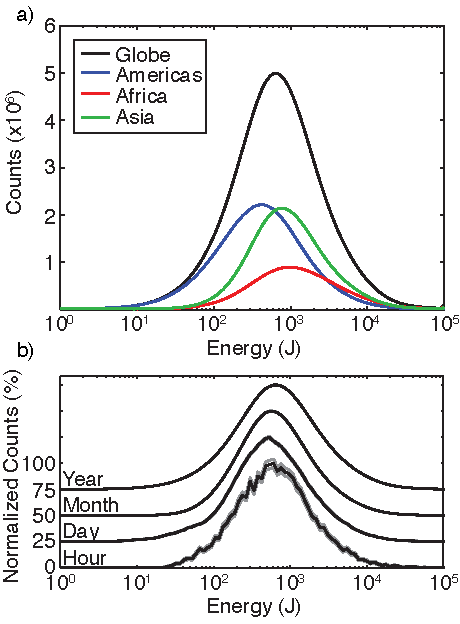
\includegraphics[scale=1]{efficiency/Figures/2012RS005049-p1.pdf}
   \caption{(a) WWLLN stroke energy distribution for the globe (black), the Americas (blue), Asia (green) and Aftica/Europe(red).
(b) WWLLN global stroke energy distribution for a year (2010), month (June 2010), day (15 June 2010), and hour (09 UTC 15 June 2010).
Grey lines are statistical count errors.}
   \label{efficiency:fig:2010_Energy}
\end{figure}

In Figure~\ref{efficiency:fig:2010_Energy}a the statistical error bars (Poisson statistics) are not plotted as they would be on the order, or smaller than, the line width.
It is important to note that the distribution of strokes in each region is lognormal \citep{Hutchins2012} with the main differences in the total strokes detected and the median energy, which is 399~J, 1101~J, and 798~J for the Americas ($-180^\circ$ E to $-60^\circ$ E), Africa ($-60^\circ$ E to $60^\circ$ E), and Asia ($60^\circ$ E to $180^\circ$ E) respectively.
An overall lower detection efficiency over Africa, particularly for low energy strokes, causes median energy to be higher than the other regions.
Along with each region the energy distribution is lognormal from an hourly time scale to the annual distribution.
In Figure~\ref{efficiency:fig:2010_Energy}b the annual lognormal distribution is shown with a monthly, daily, and hourly distribution.
It is not until the hourly distribution that the errors are noticeable, and the distribution is still fairly lognormal.

\section{Minimum Detectable Energy}

The first step in calculating the relative detection efficiency for the entire network is working out the minimum stroke energy that WWLLN can detect at a given location and time.
This process starts by finding the detection threshold at each station, converting it to an energy value at each location in the world, and then selecting the minimum detectable network energy at every location based on the minimum observable energy from each station.
Detailed examples of how this works are given next for single stations and for the network as a whole.

\subsection{Station Threshold}

At each WWLLN station the threshold for triggering on an event (and calculating the TOGA at that station) is dynamically selected depending on observed activity at that station as described in Section 5.3 of \citet{Rodger2006}.
Presently every WWLLN station automatically adjusts the triggering threshold to send an average of 3 packets per second to the central processor.
For instance, when a station is detecting many strokes, the trigger threshold at that station is raised to maintain a steady flow of sferic packets.
Since a station can only measure the electric (or magnetic) field of an event it cannot accurately discern whether a sferic comes from a nearby weak stroke or a strong distant stroke; for the case of the strongest lightning strokes the discharge could be on the other side of the Earth from the WWLLN station and still be detected.


The effect of the variable trigger threshold can be seen in Figure~\ref{efficiency:fig:Threshold}a which is a 2~-~D histogram of number of strokes with specific RMS field and UT values on 15 June 2010 for the Dunedin, New Zealand, WWLLN station ($-45.864^\circ$ N, $170.514^\circ$ E).
In Figure~\ref{efficiency:fig:Threshold}b the threshold can be seen as the lower cutoff of the triggered RMS field strength distribution, the station threshold is reconstructed hourly as the 5th percentile value (red line) of the distribution.
The threshold value varies relatively slowly over the course of the day.


\begin{figure}[ht!]
   \centering
\noindent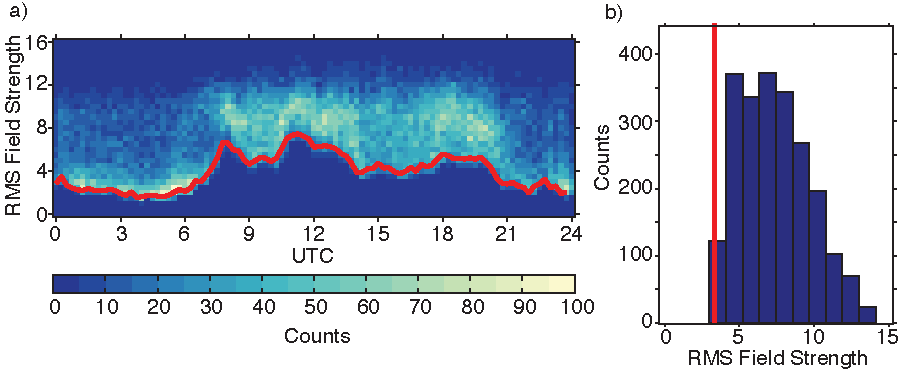
\includegraphics[scale=1]{efficiency/Figures/2012RS005049-p2.pdf}
   \caption{(a) shows the evolution of the triggered RMS field strength distribution (in arbitrary units) for the Dunedin WWLLN station with the red line showing the 5th percentile value.
(b) shows the 9 UTC slice of the distribution, with the 5th percentile value marked (red line).}
   \label{efficiency:fig:Threshold}
\end{figure}

\subsection{Station Minimum Detectable Energy}

The minimum detectable energy (MDE) is the minimum energy a lightning stroke must radiate in the VLF to be detected by WWLLN or a WWLLN station (denoted network MDE and station MDE respectively).
The MDE is a function of space, time and station threshold.
Each station has a variable threshold which varies slowly during the day.
Slow ionospheric variations can also affect the MDE by changing the VLF attenuation and detected RMS field.


Every hour the reconstructed minimum RMS field necessary to trigger an event is calculated and converted to a stroke energy.
To make this conversion the same method as calculating the radiated energy per stroke is used as described in \citet{Hutchins2012}.
This results in a station MDE for every point on a $5^\circ$ x $5^\circ$ global grid, which is the stroke energy necessary at that location to trigger a TOGA calculation at the given station.
As an example the map of the MDE for our Dunedin station (data shown in Figure~\ref{efficiency:fig:Threshold}) is shown in Figure~\ref{efficiency:fig:Threshold_Map}.
Figure~\ref{efficiency:fig:Threshold_Map} applies only to strokes detected at this one station in Dunedin, a similar map can be generated for every WWLLN station.
The high MDEs in Figure~\ref{efficiency:fig:Threshold_Map} over the Antarctic, Western Africa, and Greenland are due to the high VLF attenuation over ice, and imply that Dunedin is very unlikely to detect strokes with energy less than the MDE if they were to occur in these regions.

\begin{figure}[ht!]
   \centering
\noindent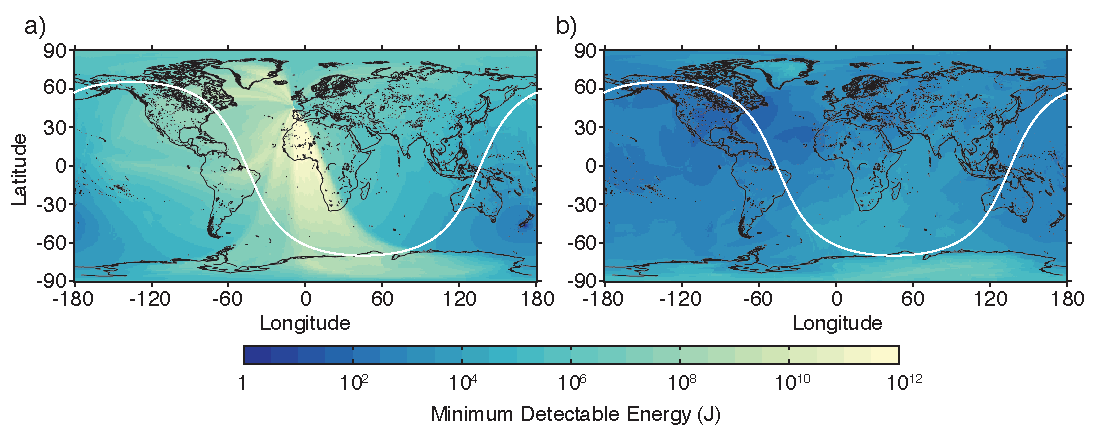
\includegraphics[scale=1]{efficiency/Figures/2012RS005049-p3.pdf}
   \caption{The minimum detectable energy (MDE) for the Dunedin station at 9 UTC on 15 June 2010.
The regions of high MDE are due to poor VLF propagation over ice from those regions to Dunedin station.
The white line shows the terminator.}
   \label{efficiency:fig:Threshold_Map}
\end{figure}

In order to locate a stroke, WWLLN requires TOGA values from at least five stations in order to conduct adequate fit error analysis.
For every $5^\circ$ x $5^\circ$ grid cell all of the minimum stroke energies from currently active WWLLN stations are ordered.
An example for one cell is shown in Table~\ref{efficiency:table:mdeTable}.
The 5th lowest from this list is used as the network MDE, because at least five stations can trigger on that energy value.
In other words, WWLLN cannot detect a stroke until it has a radiated energy which is above the trigger threshold at five or more WWLLN stations.
A map of the network MDE is shown in Figure~\ref{efficiency:fig:Minimum_Energy}.
Similar to the station MDE map for our Dunedin station, Figure~\ref{efficiency:fig:Threshold_Map}, there are higher MDE values above the Arctic and Antarctic ice regions.

\begin{table}[ht!]
\caption{Ordered list of station MDE values at $-25^\circ$N, $20^\circ$E and 09 UTC on 15 June 2010.
The fifth lowest value (in bold) is the network MDE at this location.}
\begin{center}
\begin{tabular}{p{2in}p{1in}}
\hline
Station Name 		& 	MDE (J)\\
\hline
\rule{0pt}{3ex}
Davis, Antarctica	&	34.5\\
Ascension Island	&	169.2\\
SANAE Base, Antarctica	&	193.9\\
Perth, Australia	&	2268.3\\
{\bf Rothera, Antarctica}	&	{\bf 2413.5}\\
Tel Aviv, Isreal	&	4701.1\\
. . .	&	. . .\\
Honolulu, Hawaii	&	$1.35 \times 10^8$\\
Dunedin, New Zealand	&	$5.09 \times 10^8$\\
\hline
\end{tabular}
\end{center}
\label{efficiency:table:mdeTable}
\end{table}

\begin{figure}[ht!]
   \centering
\noindent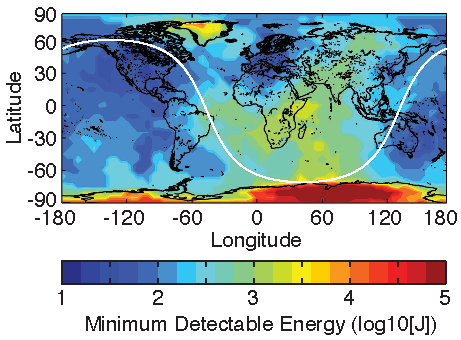
\includegraphics[scale=1]{efficiency/Figures/2012RS005049-p4.pdf}
   \caption{The minimum detectable energy (MDE) for the entire WWLLN network at 9 UTC on 15 June 2010.}
   \label{efficiency:fig:Minimum_Energy}
\end{figure}

Regions of the network with higher MDE, from either increased VLF attenuation, station thresholds or sparse coverage, preferentially detect a higher ratio of energetic strokes to all strokes.
For example southern Africa has a higher MDE than other regions and the median energy, shown in Figure~\ref{efficiency:fig:2010_Energy}a is correspondingly higher.
Conversely regions with low MDE, such as the Americas, show a lower median energy.

\section{Relative Detection Efficiency}

The next important step in calculating the relative detection efficiency is to establish the relationship between the network MDE and relative detection efficiency.
The relative detection efficiency is a measure of how well a given location in the network is being observed relative to the best region in the network.
In a given grid cell the network MDE is compared to the total WWLLN energy distribution of the past seven days.
For a given network MDE value the fraction of total strokes above the network MDE gives the relative detection efficiency.
The past seven day distribution is used as the base distribution in order to average over diurnal and station performance variations.
This lognormal base distribution is assumed to be representative of a single universal distribution of stroke energies that could be detected globally by a uniform WWLLN.

For example, if a location has an network MDE of 100~J, then the number of strokes in the past seven days above 100~J (grey area, Figure~\ref{efficiency:fig:Curve}a) is compared to the total number of strokes which were located in that location in those seven days.
In this case the grey area has a count of $2.6\times10^6$ strokes and the total number of WWLLN strokes is $2.9\times10^6$ strokes, so for this network MDE of 100~J the relative detection efficiency is 90\%.
Similarly if a location has a high network MDE value there will be few strokes with energy above it, so it will have a low relative detection efficiency.

\begin{figure}[ht!]
   \centering
\noindent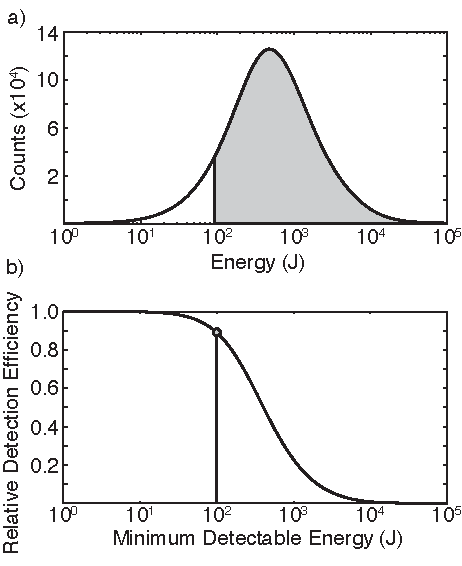
\includegraphics[scale=1]{efficiency/Figures/2012RS005049-f5.pdf}
   \caption{(a) The seven day energy distribution with the strokes above the MDE of 100~J shown in grey.
The fraction of strokes above 100~J to total strokes gives a relative detection efficiency of 0.9, shown as a circle in (b).
The fraction for all possible MDE values is shown as the curve in (b).}
   \label{efficiency:fig:Curve}
\end{figure}

This calculation is done for a range of hypothetical network MDE values which produces a curve shown in Figure~\ref{efficiency:fig:Curve}b, to give the relationship between MDE and relative detection efficiency.
This relationship is established once per day, and it is used to produce hourly maps of relative detection efficiency for that day.
This is done by taking the hourly maps of network MDE and applying this relation to every $5^\circ$ x $5^\circ$ point on the globe for every hour to convert the network MDE to the relative detection efficiency.

The relative detection values given by this process are only in reference to the energy distribution of the past seven days as seen by WWLLN.
If a region has a relative detection efficiency of 100\% then the region is able to detect all of the detected stroke energies present in the 7-day network energy distribution.
The corrections from the relative detection efficiency maps can be used to generate lightning density distributions as though WWLLN had global uniform coverage at the same level as that of the best parts of the network.
This is because the method does not correct the network to absolute stroke counts, just to a globally uniform performing WWLLN.

\subsection{Hourly Maps}

A set of four hourly maps from 15 June 2010 showing the networks relative detection efficiency every 6 hours from 00~UTC to 18~UTC is presented in Figure~\ref{efficiency:fig:Hour_Maps}.
Stations that were operational for the hour shown are displayed in white and stations that were not operational are black (operational taken to triggering $>500$ strokes/hour).
The four major competing effects on the detection efficiency are the day/night terminator, local stroke activity, station density, and station performance.
The day/night terminator effect can be seen as it moves from 00~UTC (Figure~\ref{efficiency:fig:Hour_Maps}a) through 18~UTC (Figure~\ref{efficiency:fig:Hour_Maps}d).
An increase in local stroke activity in North American afternoon (Figure~\ref{efficiency:fig:Hour_Maps}a) causes a decrease in detection efficiency as nearby stations raise their triggering thresholds.
Station density is coupled with station performance, since when a station is not operating optimally it has a similar effect as removing that station, the effect of station performance is discussed in a later section.

\begin{figure}[ht!]
   \centering
\noindent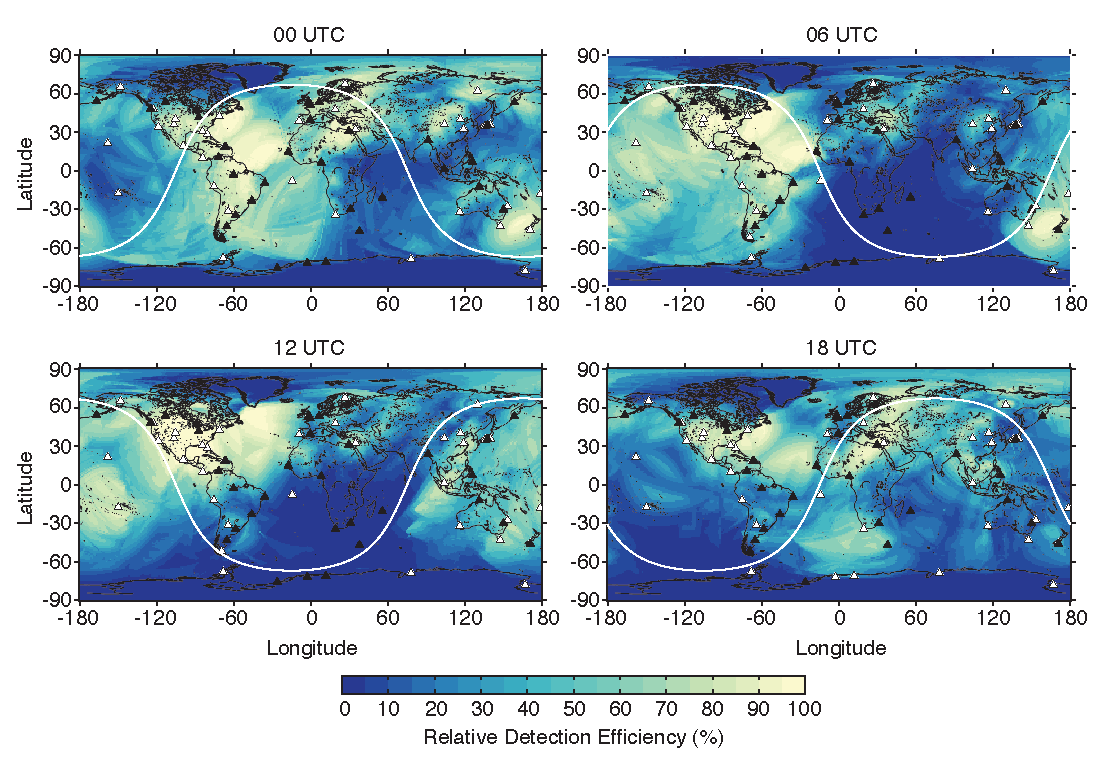
\includegraphics[scale=1]{efficiency/Figures/2012RS005049-p6.pdf}
   \caption{Relative detection efficiency maps for 00, 06, 12, and 18 UTC on 15 June 2010.
Stations are shown as triangles with operational stations in white and non-operational in black.
The minimum value of detection efficiency is set at 5\% to prevent unphysical corrections.}
   \label{efficiency:fig:Hour_Maps}
\end{figure}

Figure~\ref{efficiency:fig:Daily_Map} shows the daily relative detection efficiency from the average of the hourly maps, here grey stations were only operational part of the day.
This average map is more representative of the relative detection efficiency for the day and it shows behavior that is expected based on the distribution of stations: lower detection efficiency over most of Africa with higher detection efficiency over and around the Pacific and North America.
The low detection efficiency over Antarctica, parts of Siberia, and Greenland are due to the high attenuation of VLF propagating subionospherically over ice.
Conversely the high detection efficiency over North America, Western Europe, and Oceania, are due to the high station density and low attenuation of VLF over ocean.
In order to prevent unphysical overcorrections, a minimum relative detection efficiency of 5\% has been set for all of the relative detection efficiency maps.

\begin{figure}[ht!]
   \centering
\noindent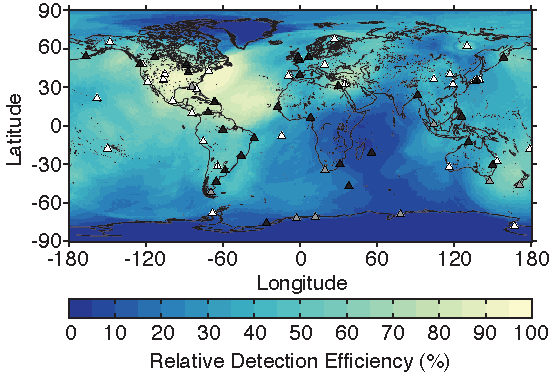
\includegraphics[scale=1]{efficiency/Figures/2012RS005049-p7.pdf}
   \caption{Daily average relative detection efficiency for 15 June 2010.
Stations are shown as triangles with operational stations in white, non operational in black, and operational for part of the day in grey.
The minimum value of detection efficiency is set at 5\% to prevent unphysical corrections.}
   \label{efficiency:fig:Daily_Map}
\end{figure}

\section{Analysis}

\subsection{Distribution Changes}

As shown in the previous sections the relative detection efficiency values in a given day are derived from the WWLLN observed stroke energy distribution from the previous seven days, this allows for direct comparisons within a day and for nearby days, but it does not take into account the changing distribution from changes in the network.
As more stations are added to the network additional low-energy strokes will be detected and the overall energy distribution will shift towards lower values.
When the overall network distribution changes between years, then for a given region the relative detection efficiency can change even if that region of the network has detected the same distribution of strokes.

One way to examine the change in the distribution of energy is to examine the temporal variability of the median of the global WWLLN energy distribution.
The median of the seven day distribution is shown in Figure~\ref{efficiency:fig:MedianEnergy}.
The median energy varies from the three year median by 52\% with the daily median value ranging from 400~J to 2000~J.
The variability is caused by ionospheric changes not accounted for in the ionospheric model used.
Several jumps in the median energy (e.g., Dec 2009 and Dec 2010) are caused by changes in the primary calibrated WWLLN station (see \citet{Hutchins2012}) such as gain changes.
The slow increase to Aug 2011 was due to a change of the primary calibrated station from the Dunedin, New Zealand station to the Scott Base, Antarctica station.
It is important to note that since the detection efficiency is relative to the past seven days, the relatively slow changes in median energy do not strongly affect the detection efficiency and highlight how the relative detection efficiency cannot correct for absolute overall network performance.

\begin{figure}[ht!]
   \centering
\noindent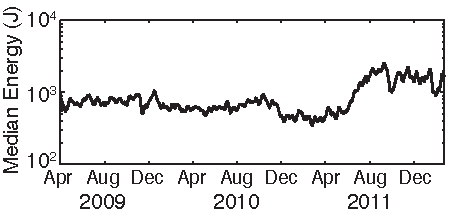
\includegraphics[scale=1]{efficiency/Figures/2012RS005049-f8.pdf}
   \caption{Median stroke energy of the 7-day distribution observed by WWLLN.
The relative detection efficiency of the network is based on this 7-day energy distribution.
   Systematic changes in median stroke energy result from unaccounted for gain changes at the primary calibrated WWLLN station (see Chapter~\ref{thesis:chapter:energy}).}
   \label{efficiency:fig:MedianEnergy}
\end{figure}

\subsection{Temporal Variability}

The evolution of the network can be seen as an increase in the global average relative detection efficiency, calculated by averaging all grid cells of each hourly map for a day.
While no region can have a relative detection efficiency over 100\%, as regions improve with more stations they will approach 100\% and increase the global average detection efficiency.
The global average relative detection efficiency from April 2009 through October 2011 is shown as the green line in Figure~\ref{efficiency:fig:DE_Evolution}.
In the Figure the total number of operational stations is shown as the black line, and it has a strong correlation to the global averaged detection efficiency with a correlation value of 0.86.
With more stations strategically added to the network the 7-day energy distribution will also change to include more low energy strokes and increase the average relative detection efficiency.


\begin{figure}[ht!]
   \centering
\noindent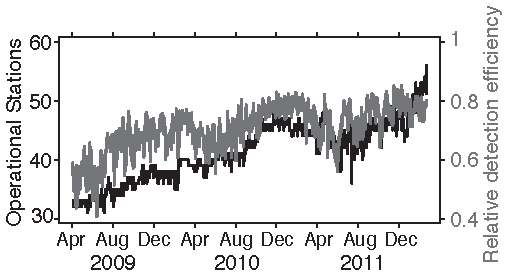
\includegraphics[scale=1]{efficiency/Figures/2012RS005049-p9.pdf}
   \caption{The number of WWLLN stations operating (black) and the global average relative detection efficiency (green) for April 2009 through October 2011.}
   \label{efficiency:fig:DE_Evolution}
\end{figure}

While Figure~\ref{efficiency:fig:DE_Evolution} shows an overall increase in the number of network stations and hence detection efficiency, Figure~\ref{efficiency:fig:deTrendLocal} shows similar curves for just low-latitude regions ($-30^\circ$ N to $30^\circ$ N, blue), a single location near Florida (at $-85^\circ$E, $30^\circ$N, red), and a single location near South Africa (at $25^\circ$E, $-20^\circ$N, green).
Removing high latitude regions, which have small contributions to lightning, increases the overall detection efficiency but does not change the overall upward trend shown by the blue curve in Figure~\ref{efficiency:fig:deTrendLocal}.
When the region near Florida is examined it can be seen that it remains fairly close to 1.0 for the entire dataset, with downward trends during local summer months due to increased local lightning activity.
The region near South Africa has a steady increase in detection efficiency except during a large drop out which occurred in the middle of 2011, caused by one of the African stations going offline.
This shows the global detection efficiency tracks the network as a whole, but it cannot be used as an accurate proxy for smaller spatial scales.

\begin{figure}[ht!]
   \centering
\noindent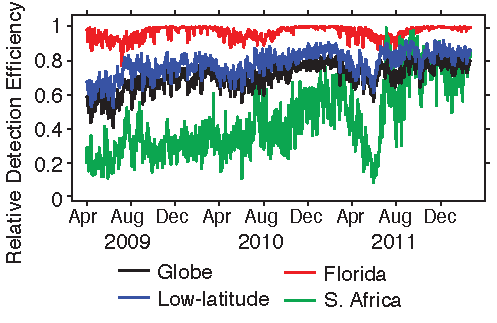
\includegraphics[scale=1]{efficiency/Figures/2012RS005049-p10.pdf}
   \caption{Daily variation of average detection efficiency for the globe (black), low-latitudes ($-30^\circ$ N to $30^\circ$ N, blue), over Florida (at $-85^\circ$E, $30^\circ$N, red), and over South Africa (at $-25^\circ$E, $-20^\circ$N, green).}
   \label{efficiency:fig:deTrendLocal}
\end{figure}

The local time variability over the region near Florida is shown in black in Figure~\ref{efficiency:fig:deUTC} and shows a total variability of about 4.9\%.
The largest drop in the relative detection efficiency occurs in the afternoon, near the peak in local lightning activity at 3pm.
This drop is due to the nearby stations raising their detection threshold in response to detecting more local strokes.
For this location the effects of local activity dominates over the expected day/night effect due to changes in VLF propagation.

\begin{figure}[ht!]
   \centering
\noindent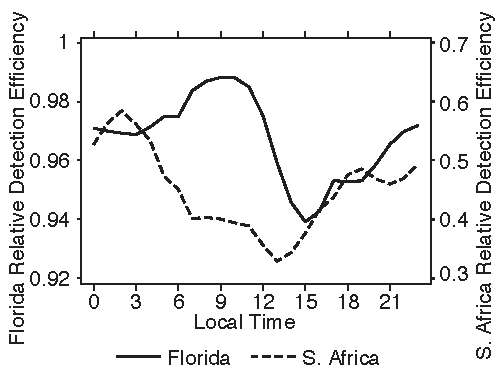
\includegraphics[scale=1]{efficiency/Figures/2012RS005049-f11.pdf}
   \caption{Average local time variation of detection efficiency over Florida ($-85^\circ$E, $30^\circ$N, solid) and South Africa ($-25^\circ$E, $-20^\circ$N, dashed), from 2009-2011.}
   \label{efficiency:fig:deUTC}
\end{figure}

The variability for the region near South Africa is shown as the dotted line in Figure~\ref{efficiency:fig:deUTC}, there is a total variability of 25.5\%.
There is an overall decrease in relative detection efficiency during the day when the sferics are propagating over the continent.
The best relative detection efficiency occurs in the middle of the night when the stations in Africa have less nearby activity and sferics are able to propagate more readily under a night ionosphere.
Compared to the Florida region there is a much higher dependence on day and night conditions as well as a much wider range of variability.

\subsection{Station Outage Effects}

While the overall performance of the network trends along with the total number of stations, a single station turning on or off can affect a large region with only a small effect on the network as a whole.
To test the influence of single stations a day of data was randomly selected, 16 June 2010, and the entire data were reprocessed with just the Honolulu, Hawaii station ($-158^\circ$E, $21^\circ$N) removed from the raw data and again with just the Maitri, Antarctica station ($12^\circ$E, $-71^\circ$N) removed.
The maps of the daily average with and without these stations are shown in Figure~\ref{efficiency:fig:scrubMap}.
For Hawaii the change is fairly local to its region in the Northeast Pacific Ocean, but leads to little effect across the entire network.
In the case of Maitri there is a larger effect since it is located in a region of sparse detector coverage and covers much of the southern Atlantic.

\begin{figure}[ht!]
   \centering
\noindent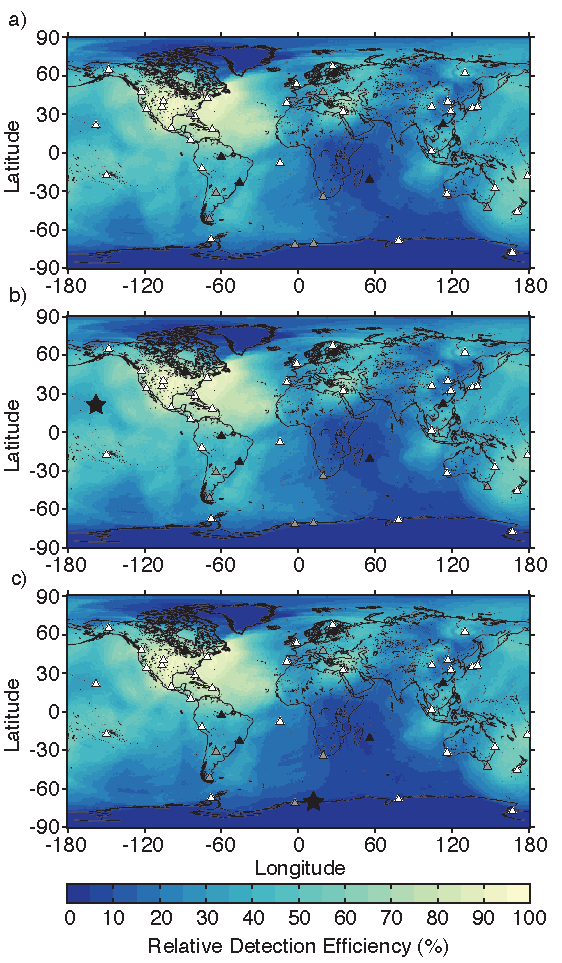
\includegraphics[scale=1]{efficiency/Figures/2012RS005049-p12.pdf}
   \caption{Relative detection efficiency map of 16 June 2010  for (a) the complete network, (b) the network with the Hawaii station (black star, $-158^\circ$E, $21^\circ$N) removed, and (c) the network with Maitri station (black star, $12^\circ$E, $-71^\circ$N) removed.
Stations are shown as triangles with operational stations in white, non operational in black, and operational for part of the day in grey.}
   \label{efficiency:fig:scrubMap}
\end{figure}

The daily average global relative detection efficiency dropped from 64\% to 63\% without Hawaii and from 64\% to 53\% without Maitri.
The detection efficiency in the grid cell over Hawaii dropped from 85\% to 78\% and from 45\% to 7.4\% in the grid cell over Maitri.
A plot of the total change between the daily averages in Figure~\ref{efficiency:fig:scrubMap} is shown in Figure~\ref{efficiency:fig:scrub}.

\begin{figure}[ht!]
   \centering
\noindent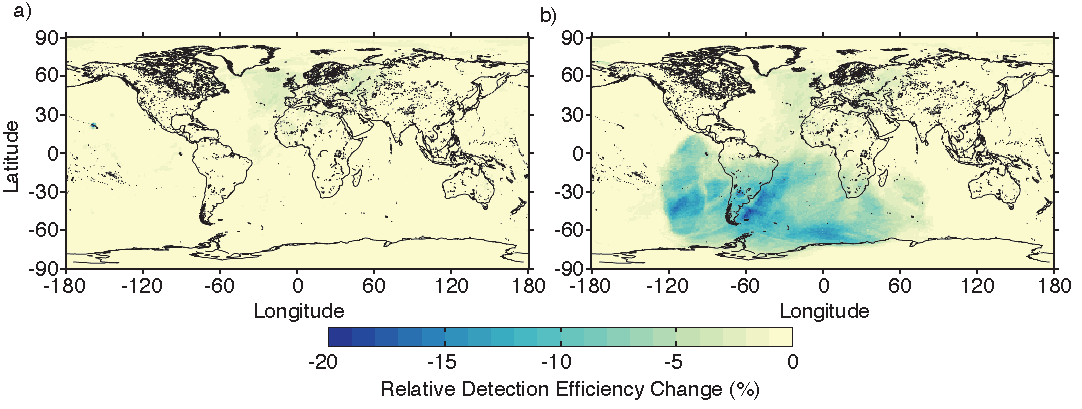
\includegraphics[scale=1]{efficiency/Figures/2012RS005049-p13.pdf}
\caption{The difference in detection efficiency for 16 June 2010 with Hawaii (a) and Maitri (b) stations completely removed from processing.}
\label{efficiency:fig:scrub}
\end{figure}

\section{Results}

The detection efficiency model can be applied to global maps of stroke density to estimate, or correct for the global stroke density which would be seen if WWLLN had a uniform spatial and temporal coverage.
This does not correct for the overall absolute detection efficiency (11\% for CG flashes in the United States, see \citet{Abarca2010}), rather it corrects for the areas with less WWLLN coverage.
The hourly stroke density plots are corrected by dividing the counts in each grid cell by the relative detection efficiency of that cell.
For example a grid cell with 100 strokes and an efficiency of 80\% would be corrected to 125 strokes.
The stroke density from 2011, Figure~\ref{efficiency:fig:Global2011}a, had the model corrections applied hourly with the condition that a 5$^\circ$ x 5$^\circ$ grid cell needed at least two strokes to have a correction applied.
A second condition was that a minimum relative detection efficiency of 5\% was set for the model.

\begin{figure}[ht!]
   \centering
\noindent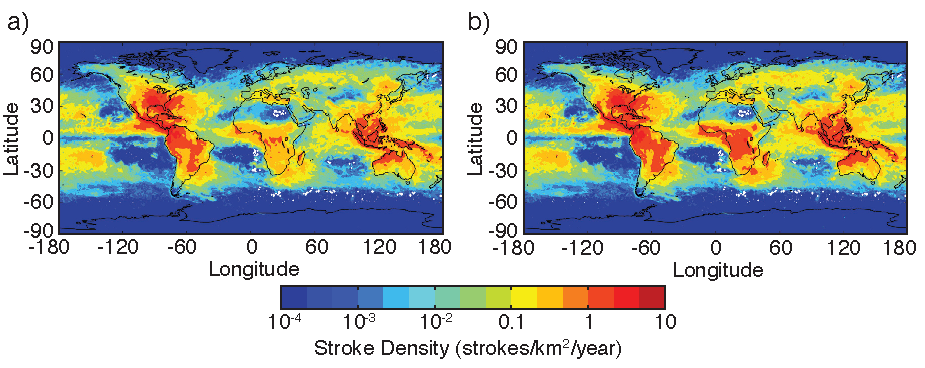
\includegraphics[scale=1]{efficiency/Figures/2012RS005049-p14.pdf}
   \caption{a) The raw 2011 global stroke density measured by WWLLN.
   b) The 2011 global stroke density corrected with the relative detection efficiency model of the network.}
   \label{efficiency:fig:Global2011}
\end{figure}

The total number of strokes for 2010 was $1.4\times10^8$ (4.4 strokes/second), and after applying the model the total was $2.0\times10^8$ strokes (6.3 strokes/second).
In 2011 the total number of strokes was $1.5\times10^8$ (4.8 strokes/second) with a model-corrected value of $1.9\times10^8$ (6.0 strokes/second).
In 2010 63\% of the global area between $\pm60^\circ$ latitude had a relative detection efficiency of at least 80\% and in 2011 this area increased from 66\% to 72\%.
If we assume that the global lightning flash rate was a constant 46 flashes/second as determined by satellite measurements using the Optical Transient Detector and Lightning Imaging Sensor \citep{Cecil2011, Christian2003} for both years, this would imply a corrected global absolute detection efficiency for cloud to ground and in-cloud flashes of 13.7\% for 2010 and 13.0\% in 2011.
The slight decline in overall detection efficiency in 2011 compared to 2010 is likely caused by the temporay decrease in the number of operational WWLLN stations during 2011, seen in Figure~\ref{efficiency:fig:DE_Evolution}.

The corrected yearly density is shown in Figure~\ref{efficiency:fig:Global2011}b, aside from the overall increase in number counts the important feature is the relative count rates over the US, Africa, and Southeast Asia.
In the uncorrected Figure~\ref{efficiency:fig:Global2011}a the peak stroke density in Asia and America are similar while Africa is about $\sim$1-10\% of these values (also shown in Figure~\ref{efficiency:fig:2010_Energy}a).
In the corrected maps we can see that the peak density in Africa is much closer in magnitude to that seen for America and Asia, and the relative densities match the distributions seen by OTD (see Figure~\ref{efficiency:fig:Christian2003}, from \citet{Christian2003} Figure 4).
The total increase in stroke counts is shown in Figure~\ref{efficiency:fig:Global2011Diff} with the greatest increases occurring over land, in particular central Africa.

\begin{figure}[ht!]
   \centering
\noindent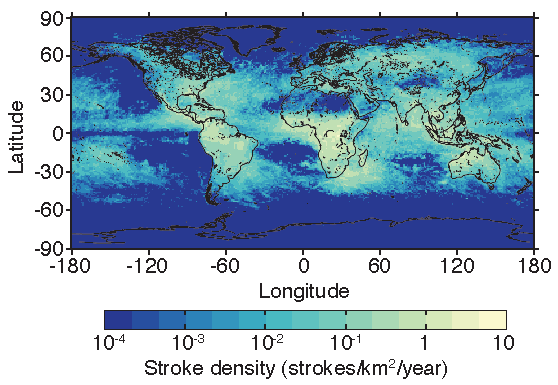
\includegraphics[scale=1]{efficiency/Figures/2012RS005049-p16.pdf}
   \caption{The increase in stroke density due to the relative detection efficiency corrections for 2011.
Uncorrected and corrected stroke densities shown in Figure~\ref{efficiency:fig:Global2011}a and~\ref{efficiency:fig:Global2011}b respectively.
The increase is plotted on the same scale as the previous two figures.}
   \label{efficiency:fig:Global2011Diff}
\end{figure}

\begin{figure}[ht!]
   \centering
\noindent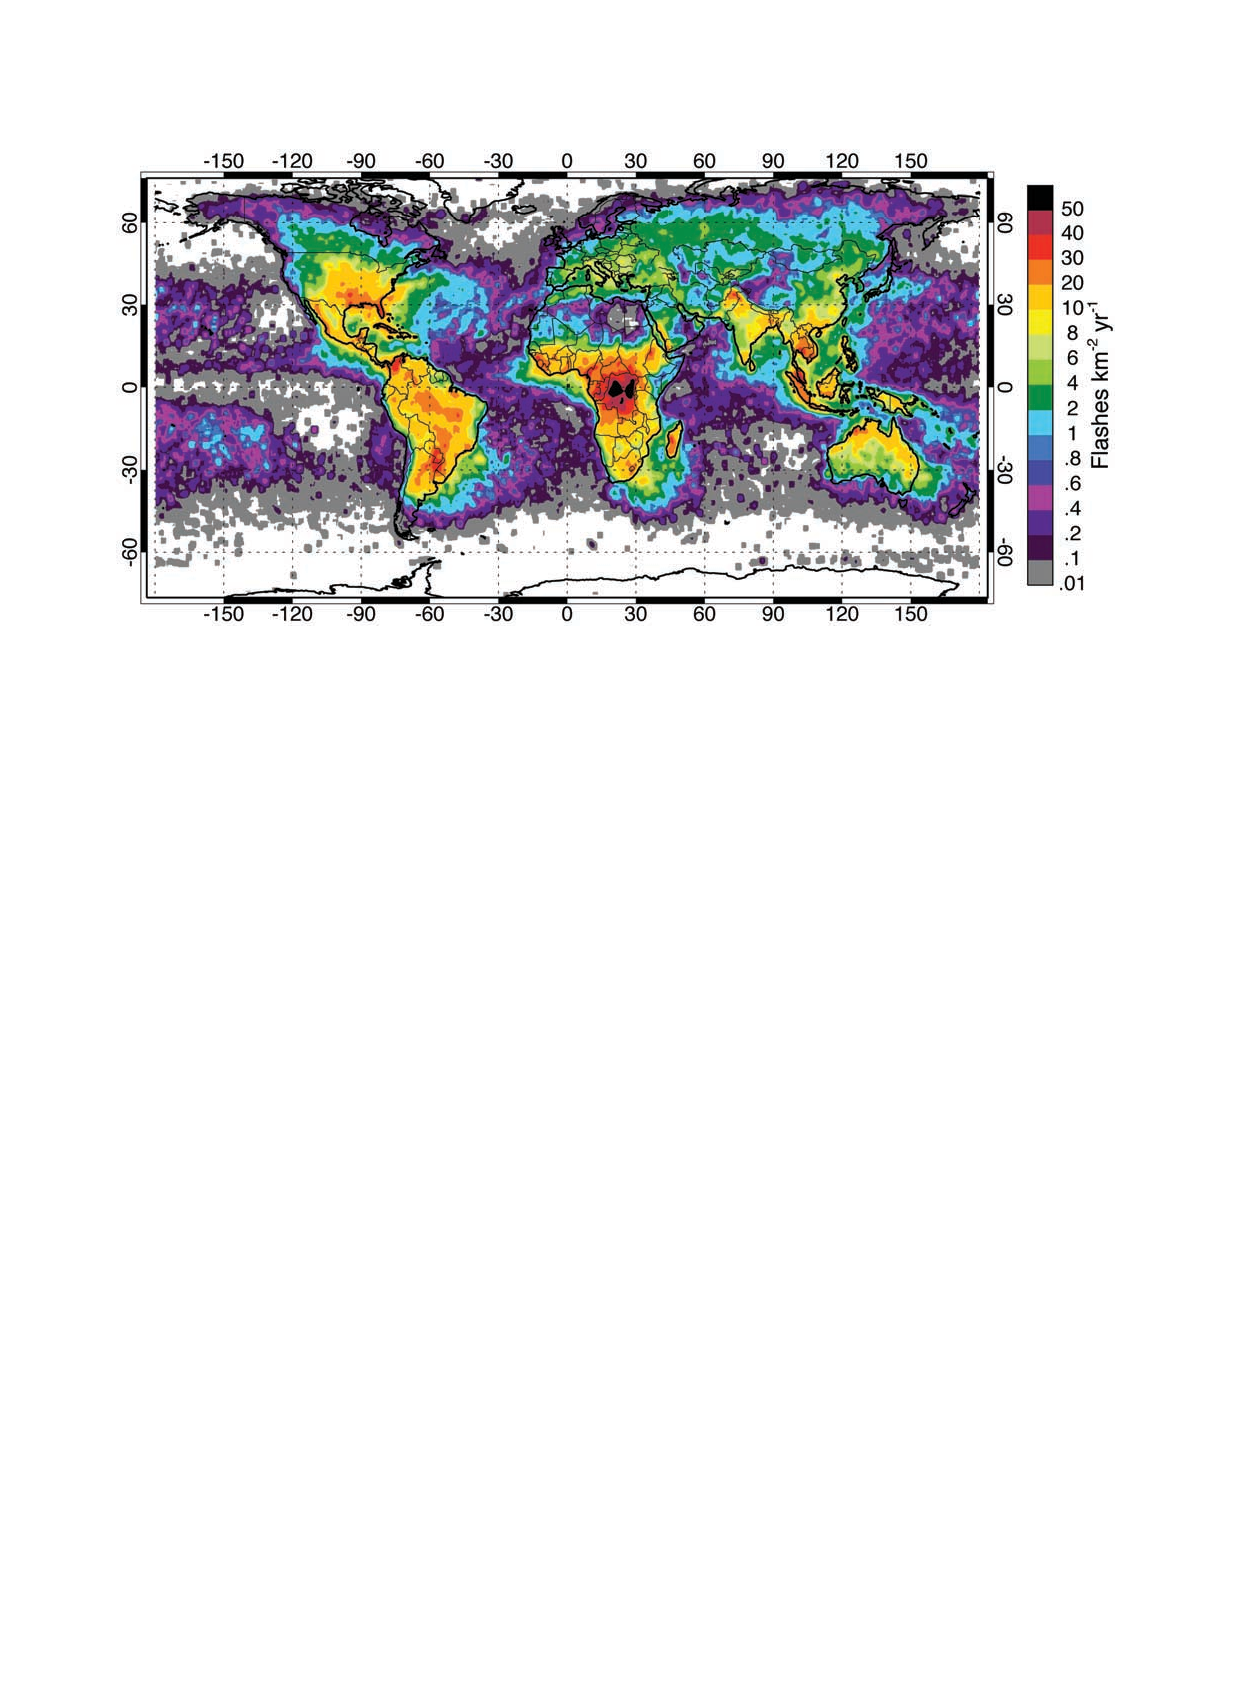
\includegraphics[scale=0.75]{efficiency/Figures/christian2003_map.pdf}
   \caption{The  distribution of lightning activity from 5 years of the Optical Transient Detector.
   Adapted from \citet{Christian2003} Figure~4.}
   \label{efficiency:fig:Christian2003}
\end{figure}

\section{Conclusion}

A relative detection efficiency model is developed for WWLLN based on the WWLLN observed stroke energy distribution.
The model is examined on various temporal scales as well as performance changes due to station outage effects.
The model is applied to the 2011 WWLLN dataset to produce a corrected map of stroke activity, matching the satellite optical flash incidence distribution.
Work on comparing distant regions is now possible as the network data can be corrected to a uniform global level of performance.

The model developed can be used for other lightning detection networks given similar operations.
Another network would need some way to determine the detection threshold at each stations, an available propagation model, and a measure of the stroke (or flash) strength.
WWLLN uses the triggering threshold at each station as reported in the TOGA packets, the LWPC model, and the energy of each stroke.